\chapter{Comment fonctionne ce template}

\epigraph{\textit{On est trop souvent imprécis lorsqu'on fait une citation.}}{Quelqu'un, un jour.}

Dans ce chapitre je donne un bref aperçu de l'organisation du template, des packages utilisés, et des éléments modifiables pour l'adapter à votre convenance.

\section{Un template fractionné}

\subsection{Pourquoi ?}

Le template est fractionné en différents morceaux ce qui permet de compiler chaque chapitre séparément, tout en conservant la mise en page qui sera celle de la thèse finale, ce qui est très pratique si comme beaucoup de monde vous commencez par le chapitre 3 et terminez votre rédaction par l'introduction\footnote{Statistique purement spéculative inférée à partir d'un échantillon représentatif de deux individus.}, mais que vous voulez quand même voir à quoi ça ressemblera avant la fin. Toutes les citations internes au chapitre $\backslash$ref\{\} et les éléments bibliographique $\backslash$cite\{\} seront correctement interprétés, seules les citations entre chapitres resteront vides tant que l'intégralité des chapitres ne sera pas compilée en même temps.

\subsection{Comment ?}

Les différents morceaux sont les suivants :
\begin{itemize}
\item[$\bullet$] dans le dossier principal : un fichier ``preambule.tex'' qui contient toutes les commandes à insérer au tout début du document. C'est notamment là qu'on chargera tous les packages utiles qui seront décrits dans le paragraphe~\ref{chap1:sec:packages}. Ce fichier n'est pas à compiler.
\item[$\bullet$] dans le dossier principal : un fichier ``biblio.bib'' qui contient l'intégralité des références bibliographiques utilisées dans la thèse.
\item[$\bullet$] des sous-dossiers pour chaque chapitre contenant chacun un fichier ``nom\_du\_chapi\-tre.tex'' et un dossier ``Figures'' qui contient... les figures ! Ces fichiers .tex ne contien\-nent que le coeur du texte et n'ont pas vocation à être compilés directement.
\item[$\bullet$] dans le dossier principal (où se trouve ``preambule.tex''), des fichiers ``compilation\_chapitre\_X.tex'' et ``compilation\_these.tex'' qui comme leur nom l'indique, sont ceux à compiler si l'on veut obtenir un chapitre en particulier ou la thèse complète (compilation standard : PDFLatex + Bibtex + PDFLatex 2 fois).
\end{itemize}

\section{Liste des packages utilisés}
\label{chap1:sec:packages}

\subsection{Packages indispensables}

\begin{itemize}
\item[$\bullet$] Encodages des caractères :
\begin{verbatim}
\usepackage[T1]{fontenc}
\usepackage[utf8]{inputenc}
\usepackage{lmodern}
\end{verbatim}
En particulier, cela assure qu'il n'y aura pas de ligatures de faites entre deux caractères successifs (comme ``fi'' par exemple), ce qui rendrait la recherche dans le document de mots contenants ces ligatures impossible.
\item[$\bullet$] Rédiger un document en français (garantit à la fois que les noms des sections seront bien en français, mais aussi que les règles typographiques françaises seront bien respectées~\cite{frenchb}) :
\begin{verbatim}
\usepackage[french]{babel}
\end{verbatim}
(remplacez ``french'' par ``english'' si vous écrivez en anglais)
\item[$\bullet$] Gestion de la mise en page et des marges :
\begin{verbatim}
\usepackage{geometry} 
\geometry{a4paper}
\end{verbatim}
Des exemples de personnalisation des marges seront donnés dans le paragraphe~\ref{chap1:sec:exemple_geometry}.
\item[$\bullet$] Gestion des citations :
\begin{verbatim}
\usepackage{cite} 
\end{verbatim}
\item[$\bullet$] Gestion des liens hypertextes:
\begin{verbatim}
\usepackage{hyperref}
\usepackage{bookmark}
\end{verbatim}
Un exemple de personnalisation des couleurs des liens est donné dans le paragraphe~\ref{chap1:sec:exemple_hyperref}.
\end{itemize}

\subsection{Packages utilitaires mais dispensables}

\begin{itemize}
\item[$\bullet$] Choix de la ``profondeur'' de la table des matières (\textit{i.e.} quels éléments sont indiqués dedans) et la ``profondeur'' de la numérotation des sections.
\begin{verbatim}
\setcounter{tocdepth}{2} 
\setcounter{secnumdepth}{2}
\end{verbatim}
Le numéro indique le degré de profondeur souhaité : 0 = chapitre, 1 = section, 2 = subsection, 3 = subsubsection. Ici on demande donc que les subsubsection ne soient pas numérotées et n'apparaissent pas dans la table des matières (contrairement aux chapitres, sections, et subsections).
\item[$\bullet$] Gestion des symboles mathématiques :
\begin{verbatim}
\usepackage{amsmath,amssymb,amsfonts,amsthm}
\end{verbatim}
Ces packages rajoutent différents symboles et polices mathématiques fréquemment utilisés.
\item[$\bullet$] Gestion des unités :
\begin{verbatim}
\usepackage{siunitx}
\end{verbatim}
Le package a énormément d'options, pour un descriptif détaillé je vous invite à vous reporter à la documentation~\cite{siunitx}. Quelques exemples seront donnés dans le paragraphe~\ref{chap1:sec:exemple_siunitx}.
\item[$\bullet$] Gestion des figures :
\begin{verbatim}
\usepackage{graphicx}
\usepackage{caption}
\usepackage{subcaption}
\end{verbatim}
Le package ``subcaption'' permet de gérer des figures avec plusieurs sous figures (il remplace le package ``subfig'' qui n'est plus mis à jour) et requiert le package ``caption''. Un exemple est donné dans le paragraphe~\ref{chap1:sec:exemple_subcaption}.
\item[$\bullet$] Gestion des tableaux et listes :
\begin{verbatim}
\usepackage{booktabs}
\usepackage{array}
\usepackage{paralist}
\end{verbatim}
\item[$\bullet$] Gestion de la table des matières :
\begin{verbatim}
\usepackage[nottoc]{tocbibind}
\usepackage{tocloft}
\end{verbatim}
La première commande assure que la bibliographie apparaisse dans la table des matières, mais que la table des matières n'apparaissent pas elle-même dans la table des matières. La seconde permet une meilleure gestion des espacements dans la table des matières.
\item[$\bullet$] Gestion de la couleur :
\begin{verbatim}
\usepackage{xcolor}
\end{verbatim}
\end{itemize}

\subsection{Packages cosmétiques}
\begin{itemize}
\item[$\bullet$] Jolis en-têtes.
\begin{verbatim}
\usepackage{fancyhdr}
\usepackage{emptypage}
\end{verbatim}
La deuxième ligne garantit que les pages ``blanches'' (comme celle entre la table des matières et le chapitre 1 par exemple) seront réellement blanches (\textit{i.e.} sans en-tête ni pied de page). Des exemples de personnalisation seront donnés dans le paragraphe~\ref{chap1:sec:exemple_fancyhdr}
\item[$\bullet$] Jolis chapeaux de début de chapitre.
\begin{verbatim}
\usepackage[Lenny]{fncychap}
\end{verbatim}
Vous pouvez personnaliser en remplaçant l'argument ``Lenny'' par (au choix) : Sonny, Glenn, Conny, Rejne, Bjarne, Bjornstrup~\cite{fncychap}.
\item[$\bullet$] Rajout de symboles (note de musique, bullet point, etc.) :
\begin{verbatim}
\usepackage{textcomp}
\end{verbatim}
\item[$\bullet$] Possibilités de mettre des citations en début de chapitre :
\begin{verbatim}
\usepackage{epigraph}
\end{verbatim}
Un exemple est donné dans le paragraphe~\ref{chap1:sec:exemple_epigraph}.
\end{itemize}


\section{Exemples et personnalisation}

\subsection{Mise en page}
\label{chap1:sec:exemple_geometry}
La personnalisation de la mise en page peut se faire de la façon suivante :
{\small \begin{verbatim}
\geometry{%
  a4paper,                % format de papier
% Définition des marges :
  left= 3cm,            % marge intérieure à la page
  right = 2cm,          % marge extérieure
  top = 3cm,
  bottom = 3cm,
% En-tête et pied de page :
  headheight=6mm,         % espace réservé à l'en-tête dans la marge top
  %headsep=3mm,            % espace entre le corps et l'en-tête
  %footskip=9mm            % espace entre le corps et le pied de page
}
\end{verbatim}}
\noindent Dans l'hypothèse où la thèse est souvent imprimée et reliée, on a spécifié ici que les marges soient plus importantes du côté intérieur des pages.

\subsection{Choix des couleurs des liens hypertextes}
\label{chap1:sec:exemple_hyperref}

À l'aide du package ``xcolor'' on peut définir différentes couleurs, par exemple le bleu qui est utilisé pour les liens dans ce document :
{\small \begin{verbatim}
\definecolor{linkcolor}{rgb}{0,0,0.6}
\end{verbatim}}
\noindent On peut ensuite demander au package ``hyperref'' d'attribuer cette couleur (ou différentes couleurs) aux différents types de liens :
{\small \begin{verbatim}
\hypersetup{
	colorlinks=true, % colore les liens au lieu de les encadrer
	urlcolor=linkcolor, % choix de la couleur des liens URL
	linkcolor= linkcolor, % choix de la couleur des liens internes
	citecolor=linkcolor % choix de la couleur des liens de citations
}
\end{verbatim}}

\subsection{Gestion des unités avec SI-unitx}
\label{chap1:sec:exemple_siunitx}

La package ``siunitx'' gère les unités de façon uniforme sur le document (et c'est l'une des rares façon de tracer un $\mu$ droit pour les unités : \si{\micro\meter}). Par exemple, si l'on veut parler de la vitesse du son dans l'air à température ambiante au lieu d'écrire ``\$340 m.s\^{}\{-1\}\$'', on écrira ``$\backslash$SI\{340\}\{$\backslash$meter$\backslash$per$\backslash$second\}'', ce qui donnera \SI{340}{\meter\per\second}. Si l'on souhaite juste écrire le nom de l'unité sans mettre de chiffre devant, il suffit d'écrire ``$\backslash$si\{$\backslash$meter$\backslash$per$\backslash$second\}'' ce qui donnera \si{\meter\per\second}.\bigskip

Le choix du séparateur entre unité (le point médian dans l'exemple ci-dessus) se fait à l'aide de la commande suivante :
{\small \begin{verbatim}
\sisetup{inter-unit-product=\ensuremath{{}\cdot{}}}
\end{verbatim}}
\noindent Ainsi, si l'on souhaite changer le séparateur dans tout le document il suffira de remplacer ``$\backslash$cdot'' par ce qu'on veut.\bigskip

Il est possible de définir des unités personnalisées (par exemple si on a beaucoup de grandeurs en mètres par seconde, on pourra utiliser:
{\small \begin{verbatim}
\DeclareSIUnit\vitesse{\meter\per\second}
\end{verbatim}}
\noindent Et ainsi on pourra écrire : ``$\backslash$SI\{340\}\{$\backslash$vitesse\}'' ce qui donnera \SI{340}{\vitesse}.\bigskip

Il est également possible de choisir comment les incertitudes sont gérées à l'aide de la commande:
{\small \begin{verbatim}
\sisetup{separate-uncertainty=true,multi-part-units=single} 
\end{verbatim}}
\noindent Ici, il est demandé que les incertitudes soient indiquées de façon séparées de la valeur (par défaut avec un symbole $\pm$ entre les deux), et que l'unité ne soit pas répétée 2 fois (une fois pour la valeur et une fois pour l'incertitude). Si on écrit ``$\backslash$SI\{340(5)\}\{$\backslash$vitesse\}'' on obtiendra donc : \SI{340(5)}{\vitesse}.

\subsection{Sous-figures}
\label{chap1:sec:exemple_subcaption}

L'intérêt de faire des figures avec une organisation en sous-figure directement dans le code, c'est qu'on peut faire des références à chaque sous-figure directement sans avoir besoin de rajouter à la main des (a) ou (b) après sa commande $\backslash$ref\{figure\} ! Par exemple, dans la figure~\ref{intro:fig:potentials} on peut faire des renvois vers chacune des sous-figure indépendamment comme~\ref{intro:fig:potentials_OK} et~\ref{intro:fig:potentials_tilte}. Elle est obtenue à l'aide du code suivant :
{\scriptsize
\begin{verbatim}
\begin{figure}[ht!]
        \centering
        \begin{subfigure}[c]{0.5\textwidth}
                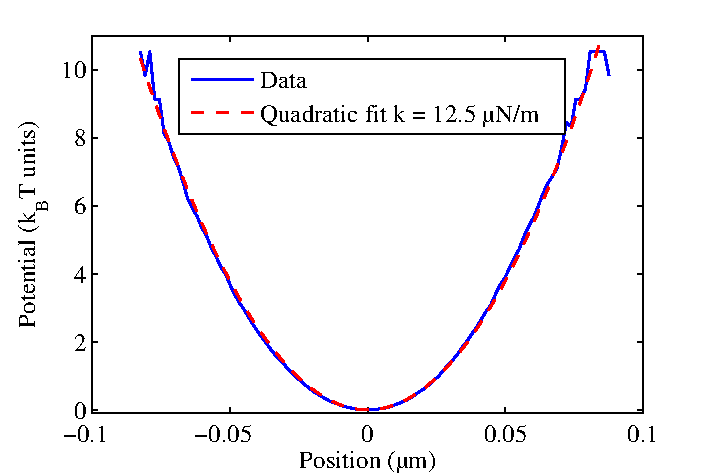
\includegraphics[width=\textwidth]{Chapitre1/Figures/exemple_potentiel_quadratic.pdf}
                \caption{A single trap}
                \label{intro:fig:potentials_OK}
        \end{subfigure}%
        %add desired spacing between images, e. g. ~, \quad, \qquad, \hfill etc.
        %(or a blank line to force the subfigure onto a new line)
        \begin{subfigure}[c]{0.5\textwidth}
                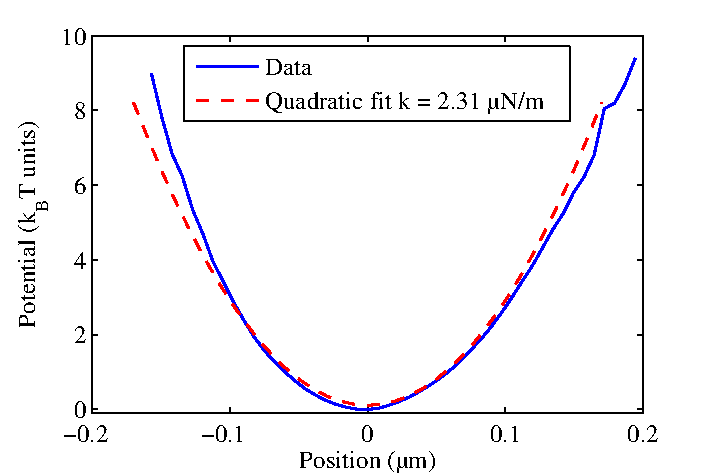
\includegraphics[width=\textwidth]{Chapitre1/Figures/exemple_potentiel_quadratic_tilte.pdf}
                \caption{One of two traps created by an AOD}
                \label{intro:fig:potentials_tilte}
        \end{subfigure}
        \caption{Exemple de deux figures.}\label{intro:fig:potentials}
\end{figure}
\end{verbatim}}

\begin{figure}[ht!]
        \centering
        \begin{subfigure}[c]{0.5\textwidth}
                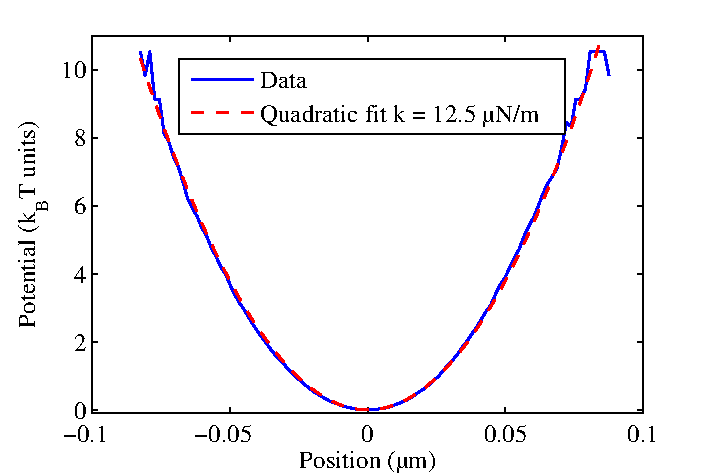
\includegraphics[width=\textwidth]{Chapitre1/Figures/exemple_potentiel_quadratic.pdf}
                \caption{A single trap}
                \label{intro:fig:potentials_OK}
        \end{subfigure}%
        %add desired spacing between images, e. g. ~, \quad, \qquad, \hfill etc.
        %(or a blank line to force the subfigure onto a new line)
        \begin{subfigure}[c]{0.5\textwidth}
                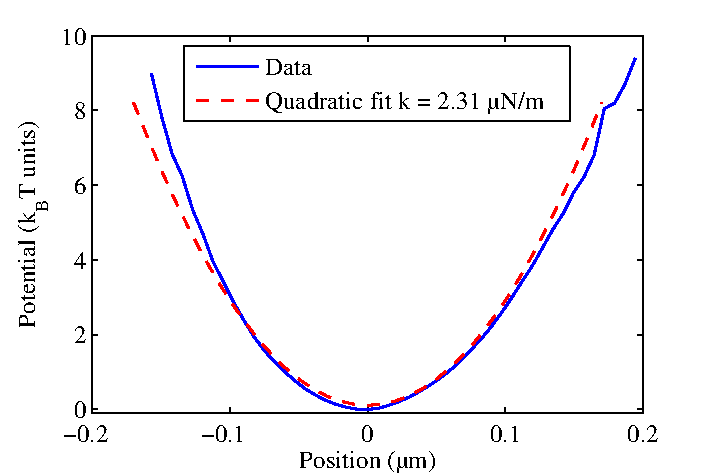
\includegraphics[width=\textwidth]{Chapitre1/Figures/exemple_potentiel_quadratic_tilte.pdf}
                \caption{One of two traps created by an AOD}
                \label{intro:fig:potentials_tilte}
        \end{subfigure}
        \caption{Exemple de deux figures.}\label{intro:fig:potentials}
\end{figure}

\subsection{En-têtes et pieds de pages}
\label{chap1:sec:exemple_fancyhdr}

Le package ``fancyhdr'' permet de choisir comment seront les en-têtes et les pieds de page. Il faut définir le style pour les pages qui sera utilisé pour la majorité des pages du document (et qui s'appelle ``fancy'') :
{\small \begin{verbatim}
\pagestyle{fancy}
\fancyhf{} % assure que les entête et pieds de page sont vides au départ
\fancyhead[LE]{\leftmark}
\fancyhead[RO]{\rightmark}
\fancyfoot[LE,RO]{\thepage}
\end{verbatim}}
\noindent Les commandes par défaut sont les suivantes :
\begin{itemize}
\item[$\bullet$] L = left, R = right, C = center, E = even pages, O = odd pages
\item[$\bullet$] $\backslash$thepage : adds number of the current page.
\item[$\bullet$] $\backslash$thechapter : adds number of the current chapter.
\item[$\bullet$] $\backslash$thesection : adds number of the current section.
\item[$\bullet$] $\backslash$chaptername : adds the word "Chapter" in English or its equivalent in the current language.
\item[$\bullet$] $\backslash$leftmark : adds name and number of the current top-level structure (for example, Chapter for reports and books classes; Section for articles ) in uppercase letters.
\item[$\bullet$] $\backslash$rightmark : adds name and number of the current next to top-level structure (Section for reports and books; Subsection for articles) in uppercase letters.
\end{itemize}
Ici on a donc demandé que : sur les pages paires en haut à gauche, on ait le nom du chapitre en cours, sur les pages impaires en haut à droite on ait le nom du paragraphe en cours, et en bas de toutes les pages on a le numéro de la page. On remarquera que par défaut les noms des chapitres, sections et paragraphes sont inscrits en majuscules dans les en-têtes, ce que je trouve personnellement assez moche. Pour y remédier, on peut redéfinir les commandes $\backslash$leftmark et $\backslash$rightmark (code à insérer avant la commande $\backslash$fancyhf{}) :
{\small\begin{verbatim}
\renewcommand{\chaptermark}[1]{\markboth{\chaptername \ \thechapter.\ #1}{}}
\renewcommand{\sectionmark}[1]{\markright{\thesection.\ #1}}
\end{verbatim}}

Il faut ensuite définir le style des pages ``spéciales'' comme celles de début de chapitre (qui s'appellera ``plain'') :
\begin{verbatim}
\fancypagestyle{plain}{
\fancyhf{}
\fancyfoot[RO,RE]{\thepage}
\renewcommand{\headrulewidth}{0pt}
\renewcommand{\footrulewidth}{0pt}}
\end{verbatim}
\noindent En particulier, il est spécifié que pour ces pages, la barre horizontale qui sépare l'en-tête du corps du texte soit d'épaisseur nulle.

\subsection{Citation en début de chapitre}
\label{chap1:sec:exemple_epigraph}

Que serait une thèse sans une citation en début de chapitre ?

\noindent Le package ``epigraph'' permet d'ajouter des citations avec la syntaxe suivante :
{\small \begin{verbatim}
\epigraph{\textit{Texte de la citation.}}{Auteur}
\end{verbatim}}
\noindent Si le résultat ne vous satisfait pas, vous pouvez également utiliser le package ``quotchap'' avec la syntaxe suivante :
{\small \begin{verbatim}
\begin{savequote}
Texte de la citation.
\qauthor{Auteur}
\end{savequote}
\end{verbatim}}

\subsection{Intégration de code}
\label{chap1:sec:exemple_code}

Que serait une thèse sans code ?

\noindent Le package ``listings" permet d'intégrer des bloc de code avec une personnalisation de la colorisation syntaxique. Pour en faire appel :
{\small \begin{verbatim}
\begin{lstlisting}
Ton code ici
\end{lstlisting}
\end{verbatim}}
\noindent Par defaut voici la syntax donnée :
\begin{lstlisting}
# Création du circuit quantique
q = QuantumRegister(nb_qubits)
c = ClassicalRegister(nb_qubits)

qc = QuantumCircuit(q, c)

# Pairing aléatoire
i = 0
while i < nb_qubits:
    cible_qbit = random.choice(random_circuit)
    qc.rx(math.pi / 2, q[cible_qbit])
    random_circuit.remove(cible_qbit)
    if len(random_circuit) != 0:
        target_qbit = random.choice(random_circuit)
        qc.cx(q[cible_qbit], q[target_qbit])
        random_circuit.remove(target_qbit)
    i += 2

qc.measure(range(nb_qubits), range(nb_qubits))
\end{lstlisting}

